\documentclass{article}

\usepackage{fullpage}
\usepackage[utf8]{inputenc}
\usepackage[american]{babel}
\usepackage{csquotes}
\usepackage{listings}
\usepackage[table]{xcolor}
\usepackage{amssymb}
\usepackage{amsmath}
\usepackage{fancyhdr}
\usepackage{lastpage}
\usepackage{parskip}
\usepackage{abstract}
\usepackage{url}
\usepackage{float}
\usepackage{enumitem}
\usepackage{fancybox}
\usepackage{amsmath}
\usepackage{graphicx}
\usepackage[bottom]{footmisc}
\usepackage{hyperref}
\usepackage{makecell}
\usepackage{ifthen}
\usepackage{listings}
\usepackage{parcolumns}
\usepackage{subcaption}
\usepackage{drawstack}

\usepackage[backend=biber]{biblatex}
\bibliography{report}
\addbibresource{report.bib}

\setcounter{secnumdepth}{3} % only chapter and sections will be numbered
\setcounter{tocdepth}{3}    % entries down to \subsubsections in the TOC

% constants
\newcommand{\COURSE}{Bachelor Thesis}
\newcommand{\TITLE}{Abstract Machine}
\newcommand{\DATE}{June 2015}

\addto\captionsamerican{\renewcommand{\contentsname}{Table of Contents}}

%%% Local Variables:
%%% mode: latex
%%% TeX-master: "report"
%%% End:

% generalized stuff
\newcommand{\code}[1]{\texttt{#1}}
\newcommand{\term}[1]{\textit{#1}}

% colors
\definecolor{Brown}{cmyk}{0,0.81,1,0.60}
\definecolor{OliveGreen}{cmyk}{0.64,0,0.95,0.40}
\definecolor{CadetBlue}{cmyk}{0.62,0.57,0.23,0}
\definecolor{lightlightgray}{gray}{0.95}
\definecolor{lightgray}{gray}{0.85}
\definecolor{sh_comment}{rgb}{0.12, 0.38, 0.18}
\definecolor{sh_keyword}{rgb}{0.37, 0.38, 0.75}
\definecolor{sh_string}{rgb}{0.06, 0.10, 0.98}

% listings
\lstset{
  basicstyle=\small\ttfamily,
  stringstyle=\color{sh_string},
  keywordstyle = \color{sh_keyword}\bfseries,
  commentstyle=\color{sh_comment},
  backgroundcolor=\color{lightlightgray},
  frame=single,
  rulecolor=\color{lightgray},
  framesep=3pt,
  numbersep=5pt,
  xleftmargin=10pt,
  xrightmargin=10pt,
  showspaces=false,
  showstringspaces=false,
  tabsize=4,
  aboveskip=5pt,
  belowskip=5pt,
  lineskip=2pt,
  captionpos=b,
  numbers=left,
  numberstyle=\tiny,
  stepnumber=1,
  numbersep=100pt,
  breaklines,
  numbersep=5pt,
  breakatwhitespace=false,
  showspaces=false,
  showtabs=false
}

 % TODO
\lstdefinelanguage{bytecode}{
  keywords={fn, pop},
  keywordstyle=\color{blue}\bfseries,
  ndkeywords={class, export, boolean, throw, implements, import, this},
  ndkeywordstyle=\color{darkgray}\bfseries,
  identifierstyle=\color{black},
  sensitive=false,
  comment=[l]{//},
  morecomment=[s]{/*}{*/},
  commentstyle=\color{purple}\ttfamily,
  stringstyle=\color{red}\ttfamily,
  morestring=[b]',
  morestring=[b]"
}

\let\oldcite=\cite
\renewcommand\cite[1]{\ifthenelse{\equal{#1}{NEEDED}}{[citation~needed]}{\oldcite{#1}}}


\pagestyle{fancy}
\fancyhf{}
\setlength{\parindent}{0pt}
\setlength{\headheight}{15pt}
\setlength{\headsep}{25pt}
\lhead{\COURSE}
\chead{\TITLE}
\rhead{\leftmark}
\cfoot{Page \thepage{} of~\pageref{LastPage}}

\begin{document}
%%% Local Variables:
%%% mode: latex
%%% TeX-master: "report"
%%% End:

\newcommand*\formatname[2]{
  \leavevmode
  \rlap{\textit{#1}}
  \hspace{0.3\linewidth}
  \code{#2}}

\begin{titlepage}

\thispagestyle{empty}

\begin{flushright}
  
\includegraphics[width=9cm]{images/dtu}
\end{flushright}

\vskip20mm
\begin{center}
  \vskip5mm
  \huge\textbf{\TITLE}
  \vskip5mm
  \Large \COURSE
  \vskip3mm
  \large \DATE
\end{center}
\vfill

\begin{flushleft}
  \normalsize
  \formatname{Markus Veie Færevaag}{s123692} \par
  \formatname{Simon Altschuler}{s123563} \par
  \vskip2cm
  
\includegraphics[width=7cm]{images/dtu-compute}
\end{flushleft}

\end{titlepage}

\clearpage

\section{Abstract}
\clearpage

\section{Acknowledgements}
\clearpage

\tableofcontents
\clearpage

\section{Introduction}
\label{sec:intro}
%%% Local Variables:
%%% mode: latex
%%% TeX-master: "../report"
%%% End:

% Motivation

New programming languages are coming into existence at a very rapid pace. Tools
for creating languages are in abundance, and even the beginning student of
computer science will most likely posses the knowledge to use them. When
languages become pass\'e or fundamental shortcomings are discovered, the
prevalent solution seems to be the creation of new and improved languages
instead of updating the existing. All of this has resulted in hundreds, if not
thousands, of available languages in a myriad of styles and paradigms for just
as many different purposes.

The world of language paradigms has become something of a religious matter for
many. Some swear by the functional approach, others by object orientation and
some insist on procedural languages, the rest on something in between. Each
require distinct and often very complex implementations that are inherently
difficult to optimize and evolve as the feature sets expand. Static or dynamic
typing is another question that divides people that of like pineapple on
pizza; strong arguments exist for both and it often comes down to a matter of
taste and preference.

Intrinsic to a language is a platform on which to be executed, be it a desktop
computer, cell phone, embedded device or essentially any other digital
device. Historically, languages where developed to be used on a single platform,
often written for a particular processor architecture, but nowadays only the
most domain specific languages can make due with that. Any language that desires
widespread adaptation must work on a multitude of devices, and not only are
there scores of architectures on the market, they are also very different in
terms of execution models and what technical primitives they provide.

Altogether language and platform diversity has grown beyond what most would have
believed when the first programmable machines appeared. That is why abstract
machines are becoming increasingly relevant to modern computer science.

In brief, an abstract machine relieves language creators of the burden of
architecture specific implementation. By providing a unified platform they
abstract away the underlying hardware specifics and can provide a higher level
of expressiveness than the bare-metal counterpart.

There are many abstract machines available today, and several are industrial
strength systems that are in use on billions of devices. What they generally
lack however, is flexibility in terms of language support. Usually they are
designed with a specific language, or family or languages, in mind which
obviously comes at the cost of adaptability by other languages. Emerging
paradigms such as dynamic and functional\footnote{Functional languages have been
  around for a long time, but are becoming increasingly popular} languages are
not well suited for the currently available abstract machines.

Having written a compiler for a functional language\footnote{In the course
  ``02122 Software Technology Project F14'' at DTU Compute} we are aware of the
issues faced by compiling code to traditional platforms, and have felt the need
for something better.

\subsection{The Multi-Paradigm Abstract Machine}

In response to the issues of today's available systems, the main ambition of
this project is to provide an abstract machine that is well suited for a
multitude of programming languages of different paradigms. Our system exposes
low level primitives that are relevant for system programming while being
efficient, expressive and secure enough as a higher level programming
environment.

To facilitate the above, an instruction set has been defined that covers the
requirements of many language paradigms in a solid, compact fashion with the
support of a corresponding execution model.

The instruction set and execution model have been implemented in the abstract
machine that we have named \thename{}.

\subsection{Status of the Implementation}

The \thename{} specification is an extensive document which covers a lot of
features. We have focused on implementing a subset of the specification that
enabled us to run simple programs and perform some benchmarking tests. Thus, the
full specification as is found in Appendix~\ref{sec:appendix:spec} is not
implemented. The Design chapter (Section~\ref{sec:design}) presents a lot of
knowledge both for abstract machines in general and specific to \thename{}, not
all of which is implemented. However, everything presented in Implementation
chapter (Section~\ref{sec:implementation}) has been developed unless otherwise
noted.

\subsection{Structure of the report}

To provide the foundational knowledge required to satisfy the ambition of the
project, Section~\ref{sec:background} describes what components make up an
abstract machine, and what existing solutions there are along with their
shortcomings. Section~\ref{sec:design} presents the design of the abstract
machine as well as the defined instruction set and a detailed explanation of the
problems we believe it solves. Section~\ref{sec:implementation} describe the
actual implementation of the machine and how we have dealt with various issues
through process.

Section~\ref{sec:evaluation} evaluates the status of the project and presents
some code analysis as well as benchmarking data.

Related work from which we have drawn inspiration is presented in
Section~\ref{sec:related-work} and finally Section~\ref{sec:project-management}
describe how we have managed the project, both technically and personally.

Throughout the report we use specific fonts for denoting \code{code} and
\instr{instruction} related names and snippets.


\section{Background}
\label{sec:background}
In this section we present the knowledge on which the rest of the thesis is
based. We give a brief overview of modern computer architectures and then start
to dissect the subject of abstract machines in more detail. Finally we present
some of the existing solutions available today that have inspired much of the
work presented in this report.

\subsection{Computer Architectures}
\label{sec:background:computer-architectures}

An architecture is what describes the organization and programming model of a
computer including the functionality provided by, and capabilities of, a
computer system\cite{clements06}. The architecture does not dictate how
individual system are constructed neither software- or hardware-wise. Virtually
all modern general-purpose computer systems are based on the von Neumann
architecture originating from papers by John von Neumann in 1945\cite{riley87},
in which he describes the design of a computing machine using now well-known
concepts such as the arithmetic unit (nowadays part of the CPU), control unit,
memory, and input/output. The structure of modern hardware machines is still
surprisingly similar to this design, even though they are vastly more powerful
and have added myriads of improvements.

To interact with such a system, a so-called instruction set is provided, which
essentially is the language that the CPU understands. It is by use of this
predefined set of actions that the programmer can control the whole machinery
and ``tell'' the computer how to perform algorithms, read from and write to
memory, communicate with peripheral devices and so on.

Modern hardware-implemented computer architectures can execute instructions
extremely fast; the Tianhe-2 super computer performs more than
$33 \cdot 10^{15}$ floating-point operations per second\cite{ieee-tianhe}! Being
this fast comes at the cost of expressiveness in the instruction set, which are
generally very low-level and specialized for a given CPU. This is where an
abstract machine becomes relevant.

\subsection{Abstract Machines}
\label{sec:background:abstract-machines}

Abstract machines are essentially computer architectures implemented in
software. They are developed and run just as regular programs which take some
input arguments and produce corresponding output, be it graphical interfaces,
textual output, network activity, etc.

To define what an abstract machine is, it helps to compare it with other similar
systems. There are many related technologies and concepts which have mixed
definitions and can stir up confusions. We present the most notable examples and
give our own broad definitions.

An \textbf{interpreter} is a program which reads high-level source code and
directly executes the code without translation into another language or native
code. Interpreters are easy to implement, but tend to suffer from slower
performance\cite{circuitstoday}. Examples include Python\footnote{The Python
  Programming Language: \url{https://www.python.org}} and Ruby\footnote{The Ruby
  Programming Language: \url{https://www.ruby-lang.org}}.

A \textbf{compiler} translates source code from one language to another without
executing anything. The target language of compilers is typically an assembly
language understood by a CPU, regardless whether it is a hardware CPU or, as is
more relevant to this thesis, an abstract CPU implemented by an abstract
machine. A abstract machine is concerned with executing code, while the compiler
translates it. Examples include the GNU Compiler Collection\cite{gnu:gcc} and
the Glasgow Haskell Compiler\footnote{The Glasgow Haskell Compiler:
  \url{https://www.haskell.org/ghc}}.


Further there is the concept of \textbf{Just-in-Time} (JIT) and
\textbf{Ahead-of-Time} (AOT) compilation which is often misunderstood as being
part of a compiler. JIT and AOT compilation is about \textit{when} compilation
takes place, not how. JIT compilers are implemented as part of abstract machines
or runtimes, and will compile an intermediate representation into native code
during run-time. For instance a language X may be compiled into language Y which
is understood by an abstract machine. Upon execution by the abstract machine,
language Y will be translated into native code and only then executed on the
hardware.

The term \textbf{virtual machine} is where some heavy debate can be sparked as
to how it relates to abstract machines. Some distinguish the terms by defining
an abstract machine to be a purely theoretical machine and virtual machine for
the corresponding implementation. Others define the virtual machine as being a
virtualization of an existing physical system and the abstract machine as being
a purely software implemented machine. For the purpose of this thesis we regard
the term ``abstract machine'' and ``virtual machine'' to cover both.

Two overarching types of abstract machines exist, that serve two very different
purposes. First there is the \textit{system} abstract machine, which is a
program that emulates a full operating system, effectively running a copy of one
operating system in another. The program which executes the guest operating
system is called a HyperVisor, which VirtualBox\footnote{Oracle VirtualBox:
  \url{https://www.virtualbox.org}} is a popular example of. The other type is
the \textit{process} abstract machine which runs like a regular program in the
host operating system and executes a single program. Typically when the
execution of the program stops, the abstract machine also exists. In this thesis
we are concerned solely with the process machine type.

\subsubsection{Components of an Abstract Machine}

The components of an abstract machine differ wildly with each implementation,
but there are common concepts that are present in most. We will briefly outline
those here, but will describe each in much more detail through
Section~\ref{sec:design} and Section~\ref{sec:implementation}.

The \textbf{instructions set} is as mentioned the language that the abstract CPU
understands. Typically each instruction has an opcode and a mnemonic name which
eases documentation, reading and writing assembly code for human beings. Further
some instructions can take arguments of varying types, e.g.~literal numbers or
strings, memory references, register names, stack indices, etc.

The \textbf{object model} defines the way in which the machine works with data,
and the memory organization of it. Classes, interfaces, methods and structures
are examples of such mechanism that aid the organization and development of
programs. We define an \textit{object} to be an entity comprised of a collection
of data fields of arbitrary kind, and potentially including methods which are
functions that are executed in the context of the data contained in the object.

Every computing system involves an \textbf{execution model} which describes how
code is executed during run-time. It includes a specification of how and where
arguments are passed to sub-routines, how values are returned from sub-routines,
how branching or jumping in the code is performed and similar operations.

\subsubsection{Stack and Register Based Implementations}
\label{sec:background:stack-vs-register}

In relation to the execution model there are generally two schools of
implementation strategy which dictates how code is written for the system.

One is the \textit{register} based implementation, in which data is handled
through registers. Values are moved between registers and instructions take
registers as arguments and typically also produce output to registers. This
model closely resembles common assembly code and thus the underlying hardware,
which can make it easier to optimize the code for execution on hardware. The
``Parrot VM'' (details in Section~\ref{sec:related-work:parrot}) is an example
of a register based abstract machine. The other model is the \textit{stack}
based implementation. As usual, implementation details differ widely from
project to project, but generally it involves a single stack (per thread)
dedicated to operations on values, passing arguments, returning values and
everything else that the machine might support. Many instructions do not accept
any arguments but rather consume values from the stack which is expected to
contain ordered values of the correct type. The ``Java Virtual Machine''
(details in Section~\ref{sec:related-work:jvm}) is an example of a stack based
abstract machine.

\begin{figure}[h]
  \centering
  \begin{subfigure}[t]{.45\textwidth}
    \begin{lstlisting}[label={lst:background:stack}, caption=Stack based addition]
push 1
push 2
add
    \end{lstlisting}
  \end{subfigure}
  \begin{subfigure}[t]{.45\textwidth}
    \begin{lstlisting}[label={lst:background:register}, caption=Register based addition]
mov r1, $1
mov r2, $2
add r1, r2, r3
    \end{lstlisting}
  \end{subfigure}
\end{figure}

Listing~\ref{lst:background:stack} shows an example of simple addition using the
stack based model. After execution of the three instructions the value
\texttt{3} will be on top of the stack and the values \texttt{1} and \texttt{2}
will have been consumed by the \texttt{add}
instruction. Listing~\ref{lst:background:register} shows the same computation
using registers, where the result is the value \texttt{3} contained in register
\texttt{r3} and the two operands remaining in \texttt{r1} and \texttt{r2}.

There is no definitive answer to which is best, it is largely a matter of
preference and style. However, research done by rewriting the Java Virtual
Machine into a register machine has shown that register machines require 47\%
less executed instructions, is 32\% faster at executing programs, but requires
25\% more code\cite{shi05}. This is probably not the general case, but it gives
an indication of the pros and cons of each.

\subsection{Advantages and Disadvantages}

As with most things, there are both strengths and weaknesses of using abstract
machines. One of the most powerful aspects is that they are by definition
platform independent; programs written for the abstract machine can run on any
platform for which an implementation of the machine exists. Given that the
machine is written in a widely supported language, such as C or C++, it means
the machine can be compiled for use on a lot of platforms. Even embedded systems
can be supported by porting the machine, and potentially by exposing only a
subset of the full instruction set archtitecture (ISA).

Another compelling thing, arguably the main advantage, is that the instruction
set provided by the abstract machine is much more expressive than regular
assembly code. The details of hardware is abstracted away from the programmer
(or compiler), and a more high-level and easy-to-use ISA is provided. However,
some abstract machines are, or were, designed for a specific language or
language paradigm, resulting in a system which is hard to use as a code
generation target for other types of languages. An example is the Java Virtual
Machine in which the underlying tools and mechanisms of the machine are not
exposed, making it difficult to fit languages outside the original paradigm into
the machinery.

It is easy to assume that abstract machines must suffer performance-wise because
of the added abstraction layer, but interestingly that is not necessarily the
case. With an added JIT compiler the performance may be as good or even better
than languages that are pre-compiled to native code\cite{mangione98,
  qwertie11}. One reason for this is that very aggressive optimization
algorithms can be implemented for the respective ISA, giving very effective
performance improvements for free regardless which platform the code will be
executed on.

\subsection{Existing Implementations}

There are scores of abstract machine implementations available, ranging from
small research projects to widely used industrial strength systems. Some of
today's most popular languages run on abstract machines, the two most well-known
being Java and C\#\cite{langpop}. We have selected some additional examples to
discuss due to their influence or otherwise interesting nature.

\subsubsection{The Java Virtual Machine}

The Java Virtual Machine (JVM) executes programs written in the Java Bytecode
format and is available on a huge amount of platforms; everything from TVs
through cell phones and media players to desktop PCs and Internet
browsers\cite{aboutjava}. JVM was developed specifically for the Java
programming language, hence the name, but due to its popularity a large amount
of other languages now target the JVM as their main run-time. Such an example,
is the Scala Programming Language~\footnote{Scala Programming Language:
  \url{http://www.scala-lang.org/}}, which is a hybrid of the object-oriented
and functional paradigm.

The JVM is a stack based machine and is heavily tied to the object-oriented
language paradigm. Most of the low-level mechanism are inaccesible through the
ISA, which forces language implementors to fit everything into the Java object
model, which is inherently object-oriented and statically typed. As a result it
is not a straightforward task to implement dynamically typed or functional
languages on the JVM. Efforts have been made to asses this, most notably the
introduction of the \texttt{invokedynamic} instruction through the Da Vinci
project (see Section~\ref{sec:related-work:jvm} for details).

\subsubsection{Common Language Runtime}

Microsoft's Common Language Runtime (CLR) is the abstract machine that executes
the Microsoft Common Intermediate Language (CIL). Like the JVM, it is stack
based and widely used on Microsoft Windows devices. An open-source port called
Mono\footnote{The Mono Project: \url{http://www.mono-project.com}} is developed
and maintained for Mac OSX and Linux systems.

The CLR is a good example of the benefits that an abstract machine can
provide. Because all languages in the .NET family (C\#, F\#, Visual Basic, etc.)
compile to CIL, interoperability between them is straightforward which means
that a library written in C\# can be utilized in F\# code as well.

Like the JVM, the CLR is object-oriented by design and consequently suffers from
the same flexibility issues.

\subsubsection{Turing Machines}

Arguably the most fundamental and influential theorical (more precisely
mathematical) abstract machines are Turing machines. First described by Alan
Turing in 1937\cite{sep-turing-machine}, they were devised to help describe what
it means for an arbitrary task to be computable. They are essentially simple
state machines which operate on a (fictional and infinite) tape of cells of
value 0 or 1, and a read-write head that can either read or write the value of
the cell currently being scanned\cite{sep-turing-machine}. The machine acts
according to transition rules which describe what action will be performed,
given a machine state and current cell value. The action can be either a read or
write, or a movement of the tape to the right or the left.

Given these simple mechanisms it is possible to perform any imaginable
computation however complex. Because of this, systems that can do so are called
Turing complete systems.

%%% Local Variables:
%%% mode: latex
%%% TeX-master: "../report"
%%% End:


\section{A Multi-Paradigm Approach}
\label{sec:design}
% Type system
%% Representation (DWARF)
%% Typed instructions
%% Run-time type checking
%% Dynamic types
%%% !!!

% Object model
%% Virtual tables

% Memory management
%% Garbage collection

% ISA

% Closures

\section{Implementation}
\label{sec:implementation}
\subsection{Core architecture}
The

\subsection{Stacks}

\subsection{Execution model}

\subsection{Binary file}

% Assembler
%% Simple parsing/emitting
%% Label calculations (offsets)

% Stack based
%% Elements are (type, value) pairs
%% Dynamically sized elements
%%% Linked list

% Object model
%% Virtual tables
%% (Un)boxing

% Execution model
%% Single stack
%% Return values as output arguments
%% No frame pointer(?)

% Binary format (ELF)
%% Sections
%% Type encoding
%% Instructions
%%% Argument encoding

% Exception handling

% Debugging information

\subsection{Analysis}
% Valgrind
% gprof?

\subsection{Testing}
% Test-Driven Development (not strictly)
% unit tests
% black box testing


\section{Evaluation}
% Assembly generation
%% Something about generating code for the machine

% Performance
%% Function calls
%% Analysis

\section{Future development}
% What's missing
% What could be different
% What would next steps be

\section{Related work}
\label{sec:related}
%%% Local Variables:
%%% mode: latex
%%% TeX-master: "../report"
%%% End:

There are other projects, previous and current, that attempt to solve the same
or similar problems as we are with \thename{}. Here we present the ones we find
most interesting and from which we have drawn inspiration.

\subsection{Parrot VM}

The Parrot Virtual Machine\footnote{\url{http://www.parrot.org}} is a project
that attempts to solve similar issues as \thename{}. Most importantly almost solely
focuses on efficient support of dynamically typed languages. Moreover it aims to
provide very flexible interoperability between any language ported to Parrot; as
the docs say: ``In theory, you will be able to write a class in Perl, subclass
it in Python and then instantiate and use that subclass in a Tcl
program.''\cite{parrot-docs}.

An interesting aspect of Parrot is that it completely hides the lowest-level
representation of executable code, called Parrot Bytecode (PBC), which is what
the virtual machine ultimately executes. Instead various layers of abstraction
are provided to ease the task of generating and reading code. One level above
PBC there is Parrot Assembly (PASM) which is more akin to regular assembly, and
provides little to no syntactic sugar. A level further up the abstraction
hierarchy there is Parrot Intermediate Representation (PIR), that is the main
language of interaction with Parrot, whether for code generating by a compiler
or authored by human beings. Compared to other interface languages for abstract
machines, it is a high-level language with constructs such as conditional
control structures, infix operators (e.g. \texttt{=}, \texttt{>},
\texttt{\&\&}), local variable and parameter declarations (effectively hiding
calling convention mechanisms), and even classes.

This hierarchy of abstraction makes it easy to port language implementations to
Parrot because a lot of the boilerplate code (calling conventions, variable
declarations, etc.) is hidden, and if fine-grained control is required PASM is
available.

Parrot uses the so-called Polymorphic Container (PMC) type that is, as the name
suggest, a polymorphic type theoretically capable of holding any type of
data. They are however by design object-oriented and class like, because
``languages that are built on top of Parrot are typically
object-oriented''\cite{parrot-docs}. A set of common PMCs are provided by
Parrot, but new ones can be implemented using a super set of C (as to ensure
efficiency).

What Parrot does not provide is an efficient platform for statically typed
languages. For instance, it offers no support for storing and retrieving type
information, which is a very significant shortcoming in terms of statically
optimized dispatches.

In summary Parrot is to dynamically typed languages, what JVM and CLR are for
statically typed languages. That means it does not bridge the gap between the
two, but merely provides facilities for the dynamic (and mostly object-oriented)
paradigm.

\subsection{JVM's \texttt{invokedynamic}}

From its inception in 1996\cite{java-1.0-press} the JVM was a very statically
typed system that did not provide any support for dynamic languages. With its
rising popularity several non-Java languages were made available for
it. Scala\footnote{\url{http://www.scala-lang.org}} and
Groovy\footnote{\url{http://groovy-lang.org}} were among the first
\textit{dynamic} languages that were designed to be run on the JVM. They handled
dynamic typing and dispatch by ``[including] wrapper type classes, using hash
tables to provide dynamic symbol resolution, and so on''\cite{friesen14}.

The Da Vinci Machine Project\cite{da-vinci} was an effort to solve the issue of
implementing dynamic language features on the JVM. It was adopted in Java 7 in
2011, with the most essential addition (in terms of dynamic language support)
being the \texttt{invokedynamic} Java Bytecode instruction. Previous to
\texttt{invokedynamic} a caller had to know the fully qualified name and type
signature of a method that it wanted to dispatch to.

With \texttt{invokedynamic} and by use of so-called method handles, it is
possible to defer the look-up of the dispatch target to run-time and do it by
providing either a class object (for static methods) or a class instance (for
instance methods) along with the types of arguments that are given. A method
handle is comparable to what is known as a function pointer in
C\cite{friesen14}, i.e. something that designates a callable entity to which
dispatches (or invocation) can be made. A method handle is looked up during
run-time. Because a method can be looked up not only by the type of the object
on which it resides, but also by the type of the arguments that it accepts, that
naturally enables \term{multimethods}, which is similar to method overloading
with the significant difference of relying on the types of arguments given
rather than the static type of the object.

%TODO: clearer and more

\subsection{Microsoft DLR and Roslyn Compiler}

% Compiler-as-a-Service
%% Also exposed API see http://stackoverflow.com/questions/7852926/microsoft-roslyn-vs-codedom
% LINQ expression trees https://msdn.microsoft.com/en-us/library/bb882637.aspx
% Interaction with other language (IronRuby, IronPython, etc. SCSS compiler was ``ported'')
% btw DLR is dead


\section{Project management}
% Risk assesment
% Agile process
%% Phases
%% Backlogs
%% Iterations
% Technical management
%% SCM

\section{Conclusion}
\label{sec:conclusion}
The problem that \thename{} attempts to solve is a complex matter that spans a
wide range of areas in the field of computer science. As a result our work on
the implementation has involved a great deal of different types of work, varying
from instruction set design and executable file formats, to efficient hash maps
and C code architecture.

Along the way we have gained a thorough knowledge of the internals of abstract
machines and code interpretation in general. We have come to realize that it is
no simple task to build a machine that is capable of expressing most of the
modern programming language paradigms in a unified manner. In addition we have
discovered the immense value and assurance that extensive tests provides.

Implementing a machine like \thename{} has been an interesting experience in
terms of working on a non-trivial and relatively low-level software project
using an agile workflow that allowed us to cope with regular changes.

We have achieved a result that can serve as evidence that the vision of
\thename{} is indeed possible. Our benchmarkings revealed that the run-time
performance in most cases is sub-optimal for practical uses, but does not fall
far behind the Java Virtual Machine is isolated cases. The general maturity of
the machine is not on par with the existing industrial strength systems, but it
does do a good job of implementing the fundamental semantics in a different way
that could be the cornerstone for future work.

%%% Local Variables:
%%% mode: latex
%%% TeX-master: "../report"
%%% End:


\newpage
\nocite{*}
\printbibliography[heading=bibintoc]

\newpage
\section{Appendices}
\label{sec:appendix}
\subsection{Running \thename{}}
\label{sec:appendix:make}

Building \thename{} is a simple matter of using the GNU Make build tool. In the
root folder containing the file \code{Makefile}, simply run the command
\code{make} to build and run the machine with the hardcoded test program.

Tests are likewise run via make using the command \code{make test}. Valgrind
analysis and gprof profiling is performed with \code{make analyze} and
\code{make gprof}, respectively.

\subsection{\thename{} Specification}
\label{sec:appendix:spec}
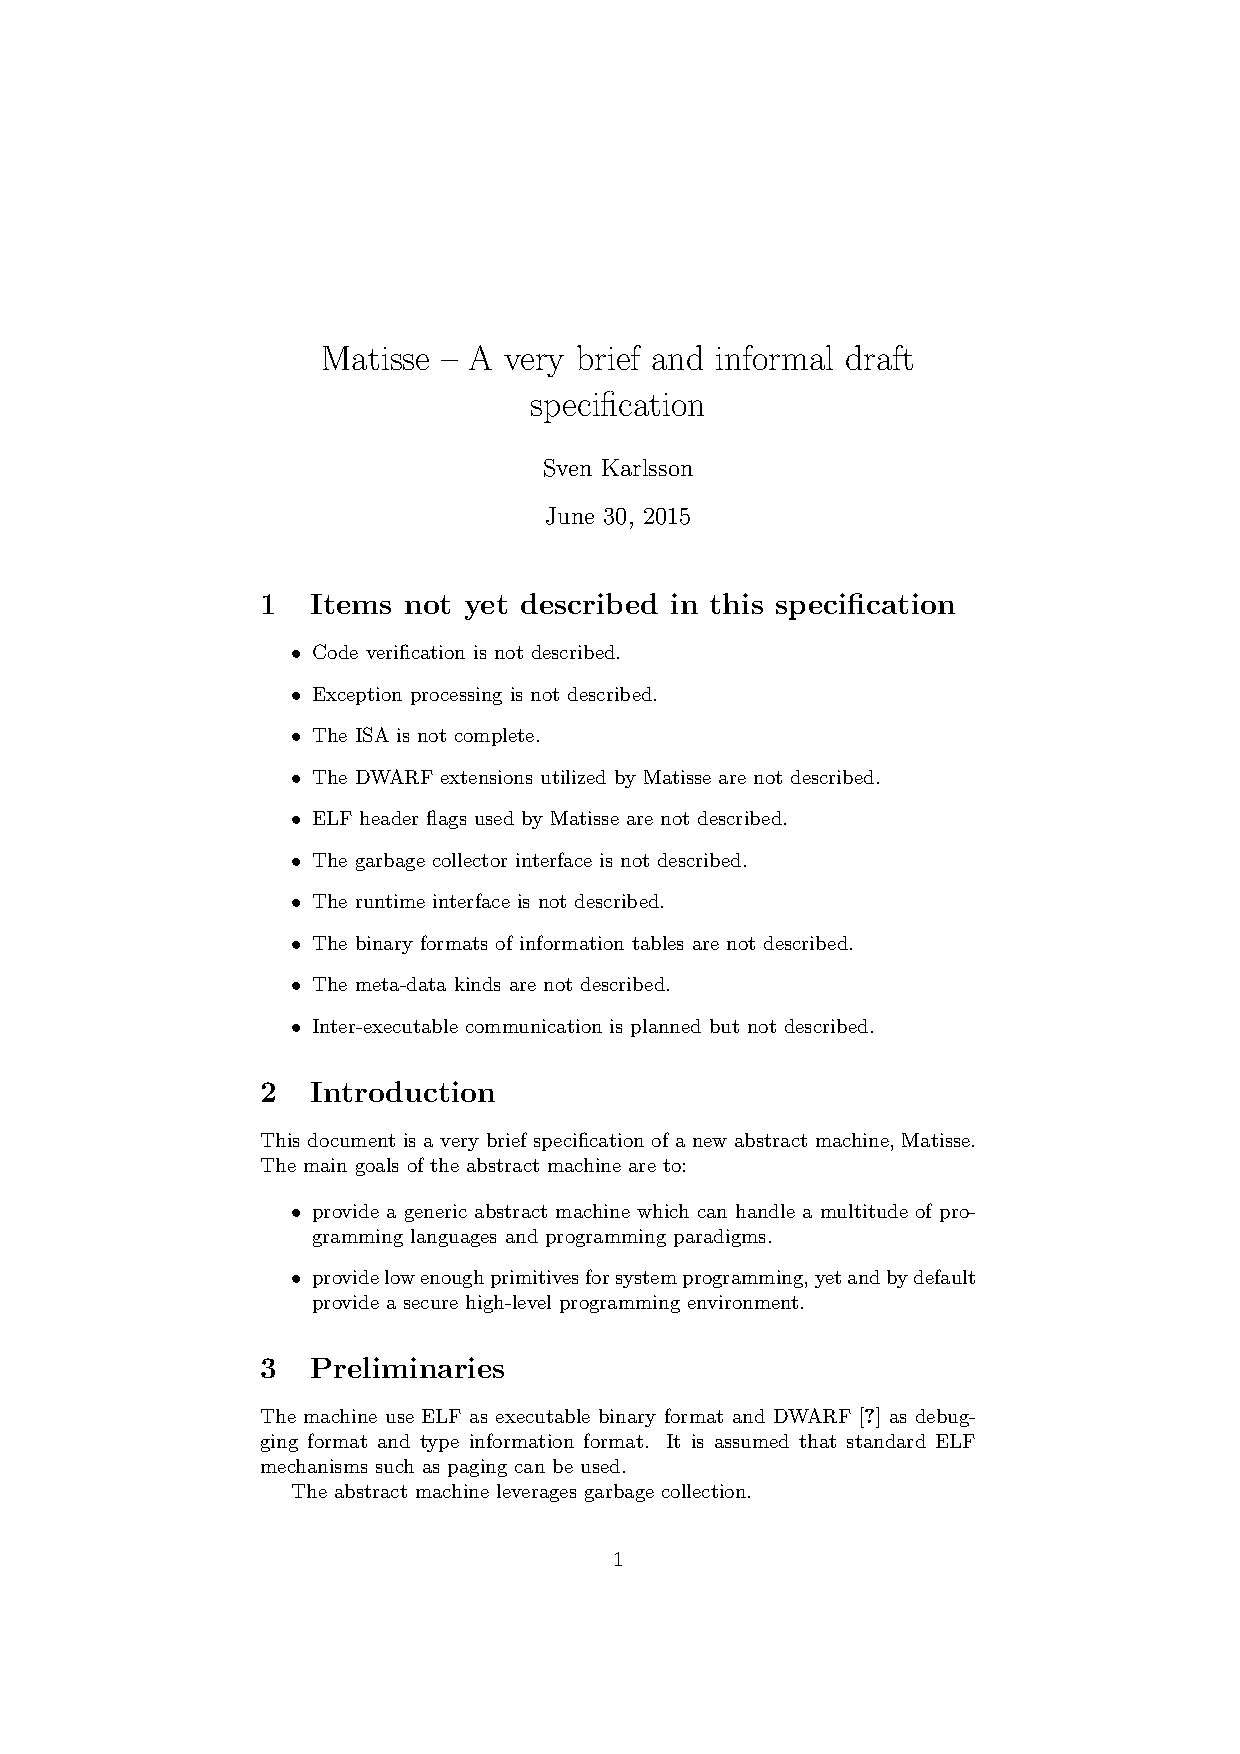
\includepdf[pages=-]{lib/spec.pdf}

\subsection{Project Inception Phase Artifact}
\label{appendix:inception-artifact}

\includepdf[pages=-]{lib/Inception.pdf}

\subsection{Benchmark Runner}
\label{appendix:benchmark}
\begin{lstlisting}[language=bash]
#!/usr/bin/bash
# benchmark runner
# based off:
# https://gist.github.com/peterjmit/3864743

repeat=1
step=1
range_from=0
range_to=30
output_file="benchmark.csv"
command=""

run_tests() {
    echo "benchmarking: ${command} ${range_from}..${range_to} (step ${step})"

    # truncate output file
    if [ -f ${output_file} ]
    then
        > ${output_file}
    fi

    # print column names
    echo "round,n,time,user,kernel" >> ${output_file}

    # repeat
    for (( j = 0; j < ${repeat}; j++ ))
    do
        # for each in range
        for (( i = ${range_from}; i < ${range_to}; i += ${step} ))
        do
            # percentage completion
            p=$(( ($i + 1) * 100 / $range_to ))
            # indicator of progress
            l=$(seq -s "#" $(($p / 2)) | sed 's/[0-9]//g')

            # time command
            /usr/local/bin/time -f "${j},${i},%e,%U,%S" -o ${output_file} -a ${command} ${i} > /dev/null

            # clear the HDD cache (i hope?)
            sync && echo 3 > /proc/sys/vm/drop_caches

            printf "%s/%s: %-48s %3s%%\r" "$(($j + 1))" "$repeat" "$l" "$p"
        done
    done

    echo -ne '\n'
}

# Option parsing
while getopts s:f:t:n:c:o: OPT
do
    case "$OPT" in
        s)
            step=$OPTARG
            ;;
        f)
            range_from=$OPTARG
            ;;
        t)
            range_to=$OPTARG
            ;;
        n)
            repeat=$OPTARG
            ;;
        o)
            output_file=$OPTARG
            ;;
        c)
            command=$OPTARG
            ;;
        \?)
            echo 'error: failed to parse args'
            exit 1
            ;;
    esac
done

shift `expr $OPTIND - 1`

if [[ $command == "" ]]
then
    echo 'error: no command to run'
    exit 1
fi

run_tests
\end{lstlisting}

%%% Local Variables:
%%% mode: latex
%%% TeX-master: "../report"
%%% End:

% Instruction set listing
% Complete backlog

\end{document}

%%% Local Variables:
%%% mode: latex
%%% TeX-master: t
%%% End:
